\section{\large \textcolor{blue}{As equações de Maxwell}}

\begin{flushleft}
\textbf{\textcolor{blue}{\Large Quest\~ao 38}}\\
\noindent

\subsection{Quest\~ao 38 IFSP 2015 - Solenoide}
Um campo magn\'etico uniforme faz um \^angulo de $30^\circ$ com o eixo de um enrolamento circular de 
300 voltas e raio de 4 cm. O m\'odulo do campo magn\'etico aumenta a uma taxa de $85\ \text{T/s}$, enquanto 
sua dire\c{c}\~ao permanece fixa. Encontre o m\'odulo da for\c{c}a eletromotriz induzida no enrolamento. 


\begin{itemize}
\item[(A)] 64 V
\item[(B)] 51 V
\item[(C)] 111 V
\item[(D)] 127 V
\item[(E)] 220 V
\end{itemize}

\vspace{0.5cm}

\textcolor{red}{\textbf{Solução:}}\\

Utilizamos a Lei de Faraday da indu\c{c}\~ao eletromagn\'etica:

\[
\mathcal{E} = N \cdot \left| \frac{d\Phi_B}{dt} \right|
\]

O fluxo magn\'etico em uma espira \'e dado por:

\[
\Phi_B = B \cdot A \cdot \cos\theta
\]

Como a dire\c{c}\~ao e a \'area permanecem constantes, temos:

\[
\frac{d\Phi_B}{dt} = A \cdot \cos\theta \cdot \frac{dB}{dt}
\]

Substituindo na express\~ao da f.e.m.:

\[
\mathcal{E} = N \cdot A \cdot \cos\theta \cdot \frac{dB}{dt}
\]

\textbf{Dados:}
\begin{itemize}
    \item $N = 300$
    \item $r = 4\ \text{cm} = 0{,}04\ \text{m} \Rightarrow A = \pi r^2 = \pi \cdot (0{,}04)^2 = 5{,}0265 \times 10^{-3}\ \text{m}^2$
    \item $\frac{dB}{dt} = 85\ \text{T/s}$
    \item $\cos(30^\circ) = 0{,}87$
\end{itemize}

Substituindo:

\[
\mathcal{E} = 300 \cdot (5{,}0265 \times 10^{-3}) \cdot 0{,}87 \cdot 85
\]

\[
\mathcal{E} \approx 1{,}3118 \cdot 85 \approx 111{,}5\ \text{V}
\]


A resposta correta é alternativa \colorbox{green!50}{\textbf{C}}.
\end{flushleft}

\noindent\rule{\linewidth}{0.6pt}\\

\begin{flushleft}
\textbf{\textcolor{blue}{\Large Quest\~ao 39 - IFSP 2015}}\\
\noindent

\subsection{Quest\~ao 39 - IFSP 2015 - Corrente de deslocamento de Maxwell}
Um capacitor de placas paralelas tem placas circulares de raio $R$ com pequena distância entre elas. 
A carga está fluindo a uma taxa de $3{,}0 \ \mathrm{C/s}$. Calcule a corrente de deslocamento de Maxwell através 
da superfície $S$ entre as placas.

\begin{figure}[!h]
\centering
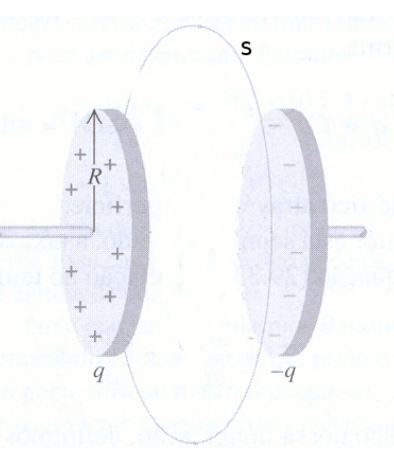
\includegraphics[scale=0.5]{figures/capacitor.png}
\end{figure}    

\begin{itemize}
\item[(A)] Zero
\item[(B)] 1,0 A
\item[(C)] 1,5 A
\item[(D)] 3,0 A
\item[(E)] 4,5 A
\end{itemize}

\vspace{0.5cm}

\textcolor{red}{\textbf{Solução:}}\\

A corrente de deslocamento de Maxwell é dada por: 

\[
i_d = \varepsilon_0 \frac{d\Phi_E}{dt}
\]

onde:
\begin{itemize}
  \item $i_d$ é a corrente de deslocamento,
  \item $\varepsilon_0$ é a permissividade elétrica do vácuo,
  \item $\Phi_E$ é o fluxo elétrico através da superfície $S$ entre as placas do capacitor.
\end{itemize}

O fluxo elétrico é definido como:

\[
\Phi_E = E \cdot A
\]

Sabemos que entre as placas de um capacitor o campo elétrico é:

\[
E = \frac{\sigma}{\varepsilon_0} = \frac{q}{\varepsilon_0 A}
\]

Logo, o fluxo elétrico será:

\[
\Phi_E = \frac{q}{\varepsilon_0}
\]

Substituindo na equação da corrente de deslocamento:

\[
i_d = \varepsilon_0 \cdot \frac{d}{dt} \left( \frac{q}{\varepsilon_0} \right) = \frac{dq}{dt}
\]

Ou seja, a corrente de deslocamento é numericamente igual à taxa de variação da carga no capacitor. Como a taxa de variação da carga é:

\[
\frac{dq}{dt} = 3{,}0 \ \mathrm{C/s}
\]

Concluímos que:

\[
\boxed{i_d = 3{,}0 \ \mathrm{A}}
\]

A resposta correta é alternativa \colorbox{green!50}{\textbf{D}}.
\end{flushleft}

\noindent\rule{\linewidth}{0.6pt}\\

\begin{flushleft}
\textbf{\textcolor{blue}{\Large Quest\~ao 35 - IFSP 2017 - Carga no capacitor}}\\
\noindent

\subsection{Quest\~ao 35 - IFSP 2017 - Carga no capacitor}
Dado o circuito composto por uma fonte de tens\~ao $V_0$, um resistor $R$, um capacitor $C$ e uma chave $S$, 
conforme apresentado abaixo. Qual express\~ao apresenta a quantidade de carga em fun\c{c}\~ao do tempo ap\'os 
a chave $S$ fechar o circuito?

\begin{center}
\begin{circuitikz}
\draw
  (0,0) to[battery, l_=$V_0$] (0,2)
  to[switch, l=$S$] (2,2)
  to[R=$R$] (4,2)
  to[C=$C$] (4,0)
  -- (0,0);
\end{circuitikz}
\end{center}

\begin{itemize}
\item[(A)] $q(t) = CV_0 \left[1 - e^{\frac{-t}{RC}}\right]$
\item[(B)] $q(t) = CV_0 \left[1 - e^{\frac{+t}{RC}}\right]$
\item[(C)] $q(t) = CV_0 \left[1 + e^{\frac{t}{RC}}\right]$
\item[(D)] $q(t) = CV_0 \left[1 + e^{\frac{+t}{RC}}\right]$
\end{itemize}

\vspace{0.5cm}

\textcolor{red}{\textbf{Solução:}}\\

Ao fechar a chave $S$ no instante $t = 0$, a corrente começa a circular no circuito RC s\'erie, carregando o capacitor. A equa\c{c}\~ao que descreve o circuito segundo a Lei de Kirchhoff das malhas é:

\[
V_0 - Ri(t) - \frac{q(t)}{C} = 0
\]

Sabendo que a corrente é a derivada da carga:

\[
i(t) = \frac{dq(t)}{dt}
\]

Substituindo:

\[
V_0 - R \frac{dq(t)}{dt} - \frac{q(t)}{C} = 0
\Rightarrow R \frac{dq(t)}{dt} + \frac{q(t)}{C} = V_0
\]

Essa é uma equa\c{c}\~ao diferencial linear de primeira ordem.

Multiplicando ambos os lados por \( C \):

\[
RC \frac{dq(t)}{dt} + q(t) = CV_0
\]

---

\textbf{Resolvendo a equação diferencial:}

Essa é uma equação linear do tipo:

\[
\frac{dq}{dt} + \frac{1}{RC} q = \frac{V_0}{R}
\]

Usamos o fator integrante \( \mu(t) = e^{t/RC} \):

\[
\frac{d}{dt} \left( q(t) \cdot e^{t/RC} \right) = \frac{V_0}{R} e^{t/RC}
\]

Integrando ambos os lados:

\[
q(t) \cdot e^{t/RC} = \int \frac{V_0}{R} e^{t/RC} dt = \frac{V_0}{R} \cdot RC \cdot e^{t/RC} + C_1
\]

\[
q(t) \cdot e^{t/RC} = CV_0 \cdot e^{t/RC} + C_1
\Rightarrow q(t) = CV_0 + C_1 \cdot e^{-t/RC}
\]

Usando a condi\c{c}\~ao inicial: \( q(0) = 0 \)

\[
0 = CV_0 + C_1 \Rightarrow C_1 = -CV_0
\]

Logo:

\[
q(t) = CV_0 \left(1 - e^{-t/RC} \right)
\]

---

\textbf{Conclus\~ao:}

A carga no capacitor em fun\c{c}\~ao do tempo \'e:

\[
\boxed{q(t) = CV_0 \left(1 - e^{-t/RC} \right)}
\]

Essa expressão mostra que a carga cresce exponencialmente com o tempo até atingir o valor máximo \( CV_0 \), com constante de tempo \( \tau = RC \).

A resposta correta é alternativa \colorbox{green!50}{\textbf{A}}.
\end{flushleft}


\noindent\rule{\linewidth}{0.6pt}\\

\begin{flushleft}
\textbf{\textcolor{blue}{\Large Quest\~ao 49}}\\
\noindent
\subsection{Quest\~ao 49 - Campo elétrico induzido por uma onda eletromagnética}
Considere uma região no espaço onde existe um campo elétrico variável no tempo, dado por $\vec{E} = E_0 \sin(\omega t) \, \hat{z},$
sendo \(E_0\) a amplitude do campo elétrico, \(\omega\) a frequência angular e \(t\) o tempo. De acordo com as equações de Maxwell, 
esse campo elétrico variável irá induzir um campo magnético também variável, dando origem a uma onda eletromagnética. Supondo que a 
onda eletromagnética se propague na direção \(+y\) e que não haja cargas livres ou correntes na região, a expressão que descreve o 
campo magnético \(B\) induzido nessa região é:


\begin{itemize}
\item[(A)] $B = \frac{ E_0}{c} \sin(\omega t) \, \hat{x}.$
\item[(B)] $B = -\frac{E_0}{c} \sin(\omega t) \, \hat{x}.$
\item[(C)] $B = \frac{E_0}{c} \cos(\omega t) \, \hat{x}.$
\item[(D)] $B = -\frac{E_0}{c} \cos(\omega t) \, \hat{x}.$
\end{itemize}

\vspace{0.5cm}

\textcolor{red}{\textbf{Solução:}}\\



\section*{1. Forma geral da onda eletromagnética no vácuo}

No vácuo, uma onda plana que se propaga na direção \(+\hat{y}\) tem os campos elétrico e magnético na forma:
\[
\vec{E}(y,t) = E_0 \sin(k y - \omega t) \, \hat{z},
\]
\[
\vec{B}(y,t) = B_0 \sin(k y - \omega t) \, \hat{x}.
\]

A relação entre as amplitudes \(E_0\) e \(B_0\) é dada por:
\[
B_0 = \frac{E_0}{c}.
\]

Considere a região do espaço onde o campo elétrico é dado por:
\[
\vec{E}(y,t) = E_0 \sin(k y - \omega t) \, \hat{z}.
\]

Queremos determinar o campo magnético associado \(\vec{B}(y,t)\), calculando o rotacional de \(\vec{E}\) e usando a \textbf{lei de Faraday}:
\[
\nabla \times \vec{E} = -\frac{\partial \vec{B}}{\partial t}.
\]

\section*{2. Cálculo do rotacional de \(\vec{E}\)}

O campo elétrico tem apenas a componente \(z\), que depende apenas de \(y\) e \(t\).  
Em coordenadas cartesianas:
\[
\nabla \times \vec{E} =
\begin{vmatrix}
\hat{x} & \hat{y} & \hat{z} \\[4pt]
\partial_x & \partial_y & \partial_z \\[4pt]
0 & 0 & E_z
\end{vmatrix}
=
\left( \frac{\partial E_z}{\partial y} \right) \hat{x} - \left( \frac{\partial E_z}{\partial x} \right) \hat{y} + 0 \, \hat{z}.
\]

Como \(E_z = E_0 \sin(k y - \omega t)\), temos:
\[
\frac{\partial E_z}{\partial y} = k E_0 \cos(k y - \omega t),
\quad
\frac{\partial E_z}{\partial x} = 0.
\]

Assim:
\[
\nabla \times \vec{E} = k E_0 \cos(k y - \omega t) \, \hat{x}.
\]

\section*{3. Lei de Faraday}

Pela lei de Faraday:
\[
\nabla \times \vec{E} = -\frac{\partial \vec{B}}{\partial t}.
\]

Logo:
\[
\frac{\partial \vec{B}}{\partial t} = -\nabla \times \vec{E} = -k E_0 \cos(k y - \omega t) \, \hat{x}.
\]

\section*{4. Integração no tempo}

Para encontrar \(\vec{B}(y,t)\), integramos no tempo:
\[
\vec{B}(y,t) = \int \frac{\partial \vec{B}}{\partial t} \, dt = -k E_0 \int \cos(k y - \omega t) \, dt \, \hat{x}.
\]

Como \(y\) é constante na derivada temporal, podemos integrar diretamente:
\[
\int \cos(k y - \omega t) \, dt = -\frac{1}{\omega} \sin(k y - \omega t).
\]

Portanto:
\[
\vec{B}(y,t) = \frac{k E_0}{\omega} \sin(k y - \omega t) \, \hat{x}.
\]

\section*{5. Relação entre \(k\), \(\omega\) e \(c\)}

No vácuo, sabemos que:
\[
c = \frac{\omega}{k} \quad \text{ou equivalentemente} \quad \frac{k}{\omega} = \frac{1}{c}.
\]

Substituindo:
\[
\vec{B}(y,t) = \frac{E_0}{c} \sin(k y - \omega t) \, \hat{x}.
\]

\section*{6. Resposta final}

Portanto, a expressão para o campo magnético induzido é:
\[
\boxed{
\vec{B}(y,t) = \frac{E_0}{c} \sin(k y - \omega t) \, \hat{x}
}
\]


A resposta correta é alternativa \colorbox{green!50}{\textbf{A}}.
\end{flushleft}

\noindent\rule{\linewidth}{0.6pt}\\

\begin{flushleft}
\textbf{\textcolor{blue}{\Large Quest\~ao 50}}\\
\noindent
\subsection{Quest\~ao 50 - Lei de Gauss para dielétricos homogêneos}
Considere uma esfera de raio \( R \) feita de um material dielétrico linear e homogêneo com permissividade elétrica \( \varepsilon \).  
Uma carga total \( +Q \) está uniformemente distribuída no volume da esfera. De acordo com a lei de Gauss, o campo elétrico \( E \) 
dentro (\( r < R \)) e fora (\( r \geq R \)) da esfera é:


\begin{itemize}
\item[(A)] $\frac{Q}{4\pi\varepsilon R^3} \, \hat{\textrm{r}} \quad \text{se} \quad r < R \quad e \quad \frac{Q}{4\pi\varepsilon_0 r^2} \, \hat{\textrm{r}} \quad \text{se} \quad r \geq R. $
\item[(B)] $\frac{Q r^2}{4\pi\varepsilon R^2} \, \hat{\textrm{r}} \quad \text{se} \quad r < R \quad e \quad \frac{Q}{4\pi\varepsilon_0 r^2} \, \hat{\textrm{r}}  \quad \text{se} \quad r \geq R.$
\item[(C)] $\frac{Q r}{4\pi\varepsilon R^3} \, \hat{\textrm{r}} \quad \text{se} \quad r < R \quad e \quad \frac{Q}{4\pi\varepsilon_0 r^2} \, \hat{\textrm{r}} \quad \text{se} \quad r \geq R.$
\item[(D)] $\frac{Q r}{4\pi\varepsilon R^2} \, \hat{\textrm{r}} \quad \text{se} \quad r < R \quad e \quad \frac{Q}{4\pi\varepsilon_0 r^2} \, \hat{\textrm{r}} \quad \text{se} \quad r \geq R.$
\end{itemize}

\vspace{0.5cm}

\begin{center}
\textbf{Superfícies gaussianas para os casos \(r<R\) e \(r\geq R\)}
\end{center}

\begin{center}
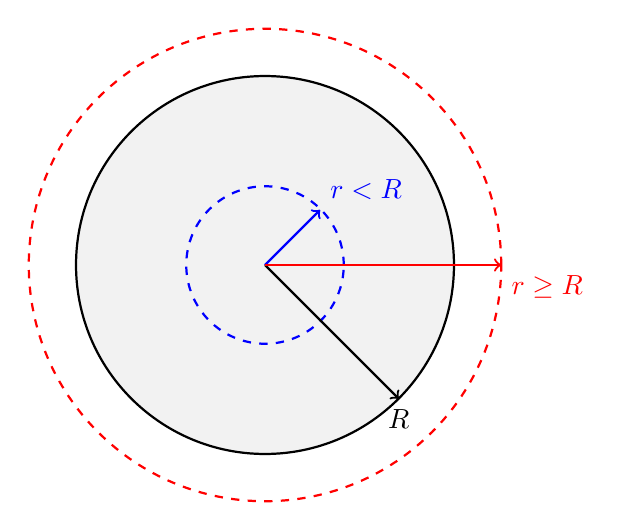
\begin{tikzpicture}[scale=2]

% Esfera carregada
\fill[gray!10] (0,0) circle (1.2);
\draw[thick] (0,0) circle (1.2);
%\node at (0,0) {\( +Q \) uniformemente distribuído};

% Superfície gaussiana interna (r<R)
\draw[dashed, blue, thick] (0,0) circle (0.5);
%\node[blue] at (0.75,0.2) {\( r<R \)};

% Superfície gaussiana externa (r>R)
\draw[dashed, red, thick] (0,0) circle (1.5);
%\node[red] at (1.7,0.2) {\( r\geq R \)};

% Marcas de raio R
\draw[thick,->] (0,0) -- (0.85,-0.85) node[below] {\(R\)};

% Raio interno
\draw[thick,->,blue] (0,0) -- (0.35,0.35) node[above right] {\(r<R\)};

% Raio externo
\draw[thick,->,red] (0,0) -- (1.5,0) node[below right] {\(r\geq R\)};

\end{tikzpicture}
\end{center}

\textcolor{red}{\textbf{Solução:}}\\

\section*{1. Densidade de carga volumétrica}

A carga está uniformemente distribuída no volume da esfera:
\[
\rho = \frac{Q}{\frac{4}{3} \pi R^3} = \frac{3Q}{4\pi R^3}.
\]

\section*{2. Lei de Gauss para dielétricos}

No material dielétrico, o campo elétrico \( \vec{E} \) está relacionado ao deslocamento elétrico \( \vec{D} \) por:
\[
\vec{D} = \varepsilon \vec{E}.
\]

A lei de Gauss para \( \vec{D} \) em forma integral:
\[
\oint_{S} \vec{D} \cdot d\vec{A} = Q_{\text{int}}.
\]

Para simetria esférica, escolhemos uma superfície gaussiana esférica de raio \( r \).  

---

\section*{3. Campo dentro da esfera (\( r < R \))}

A carga contida em uma esfera de raio \( r < R \) é:
\[
Q_{\text{int}}(r) = \rho \cdot \frac{4}{3} \pi r^3.
\]

Aplicando a lei de Gauss para \( D_r \):
\[
D_r \cdot 4\pi r^2 = Q_{\text{int}}(r) \quad \Rightarrow \quad D_r = \frac{\rho r}{3}.
\]

Como \( \vec{E} = \vec{D}/\varepsilon \), temos:
\[
E_r(r<R) = \frac{D_r}{\varepsilon} = \frac{\rho r}{3\varepsilon}.
\]

Substituindo \(\rho\):
\[
E_r(r<R) =
\frac{1}{3\varepsilon} \cdot \frac{3Q}{4\pi R^3} \cdot r =
\frac{Q r}{4\pi \varepsilon R^3}.
\]

---

\section*{4. Campo fora da esfera (\( r \geq R \))}

Para \( r \geq R \), toda a carga \( Q \) está contida:
\[
D_r \cdot 4\pi r^2 = Q \quad \Rightarrow \quad D_r = \frac{Q}{4\pi r^2}.
\]

Logo:
\[
E_r(r \geq R) =
\frac{D_r}{\varepsilon} =
\frac{Q}{4\pi \varepsilon r^2}.
\]

---

\section*{5. Resposta final}

O campo elétrico \( E_r \) em todos os pontos do espaço é dado por:
\[
\boxed{
E_r(r) =
\begin{cases}
\dfrac{Q r}{4\pi \varepsilon R^3}, & r < R \\[12pt]
\dfrac{Q}{4\pi \varepsilon r^2}, & r \geq R
\end{cases}
}
\]

A resposta correta é alternativa \colorbox{green!50}{\textbf{C}}.
\end{flushleft}

\begin{center}
\textbf{Campo elétrico \(E(r)\) em função de \(r\)}
\end{center}

O campo elétrico radial \(E(r)\) em uma esfera uniformemente carregada com raio \(R\) é dado por:
\[
E(r) =
\begin{cases}
\displaystyle \frac{Q r}{4\pi \varepsilon R^3}, & r < R \\[12pt]
\displaystyle \frac{Q}{4\pi \varepsilon r^2}, & r \geq R
\end{cases}
\]

O gráfico abaixo mostra qualitativamente o comportamento de \(E(r)\) em função de \(r\).

\bigskip

\begin{center}
\begin{tikzpicture}
\begin{axis}[
    axis lines = left,
    xlabel = {$r$},
    ylabel = {$E(r)$},
    xmin=0, xmax=2,
    ymin=0, ymax=1.2,
    xtick={0.5,1,1.5},
    xticklabels={$0.5R$,$R$,$1.5R$},
    ytick=\empty,
    domain=0:2,
    samples=100,
    width=12cm,
    height=8cm
]

% Dentro da esfera: E ~ r
\addplot[blue, thick, domain=0:1] {x};
% Fora da esfera: E ~ 1/r^2
\addplot[blue, thick, domain=1:2] {1/(x*x)};

% Linha pontilhada em r=R
\draw[dashed] (axis cs:1,0) -- (axis cs:1,1);

% Marca R no eixo x
\node[below] at (axis cs:1,0) {$R$};

\end{axis}
\end{tikzpicture}
\end{center}

\begin{flushleft}
\textbf{\textcolor{blue}{\Large Quest\~ao 27}}\\
\subsection{Quest\~ao 27 - Lei de Faraday/Lei de Ohm}
Um fio condutor em formato de armação quadrada de lado $50 \ \text{cm}$ está inicialmente em repouso dentro 
de uma região com campo magnético uniforme de $0{,}8 \ \text{T}$, perpendicular ao plano do circuito. Em determinado instante, 
o fio começa a ser puxado para fora da região do campo magnético com velocidade constante de $5 \ \text{m/s}$, de modo que a 
extremidade do quadrado atravessa a borda do campo magnético. Sabendo que o fio possui resistência elétrica de $10^{-3} \ \Omega/\text{cm}$, 
qual é a corrente elétrica induzida no circuito durante o movimento?


\begin{itemize}
\item[(A)] 3{,}0 A.
\item[(B)] 4{,}8 A.  
\item[(C)] 6{,}0 A.
\item[(D)] 8{,}2 A.
\item[(E)] 10{,}0 A.
\end{itemize}

\vspace{0.5cm}

\textcolor{red}{\textbf{Solução:}}\\

\begin{itemize}
    \item Lado do quadrado: $L = 0,5 \ \text{m}$
    \item Campo magnético: $B = 0,8 \ \text{T}$
    \item Velocidade com que a armação é puxada: $v = 5 \ \text{m/s}$
    \item Resistência linear do fio: $r = 10^{-3} \ \Omega/\text{cm} = 0,1 \ \Omega/\text{m}$
\end{itemize}

\begin{center}
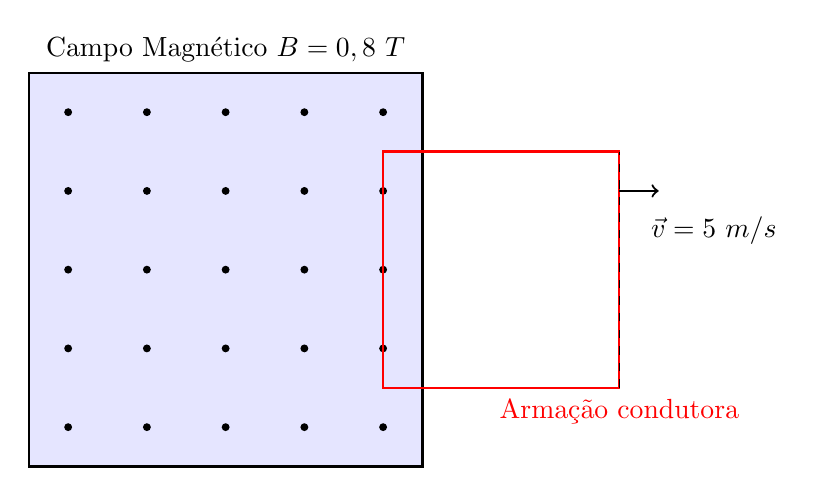
\begin{tikzpicture}

    % Área do campo magnético
    \fill[blue!10] (0,0) rectangle (5,5);
    \draw[thick] (0,0) rectangle (5,5);
    \node at (2.5,5.3) {Campo Magnético $B = 0,8 \ \text{T}$};

    % Indicação das linhas de campo magnético (pontos saindo da folha)
    \foreach \x in {0.5,1.5,2.5,3.5,4.5} {
        \foreach \y in {0.5,1.5,2.5,3.5,4.5} {
            \fill[black] (\x,\y) circle (0.05);
        }
    }
    %\node at (5.5,2.5) {Borda do campo};

    % Armação quadrada
    \draw[red, thick] (4.5,1) -- (4.5,4) -- (7.5,4) -- (7.5,1) -- cycle;
    \node[red] at (7.5,0.7) {Armação condutora};

    % Vetor velocidade
    \draw[->, thick] (7.5,3.5) -- (8,3.5);
    \node at (8.7,3.0) {$\vec{v} = 5 \ \text{m/s}$};

    % Indicação da direção de movimento da armação
    \draw[dashed] (7.5,1) -- (7.5,4);

\end{tikzpicture}
\end{center}

\textbf{1) Força eletromotriz induzida (fem):}

Durante o movimento, a variação do fluxo magnético induz uma força eletromotriz.

A \textbf{fem induzida} pode ser calculada pela expressão:

\[
\boxed{
\mathcal{E} = -\frac{d\Phi}{dt}} \quad \text{Lei de Faraday
}
\]

\[
\mathcal{E} = B \cdot L \cdot \frac{dx}{dt}
\]

\[
\mathcal{E} = B \cdot L \cdot v
\]

Onde:

\begin{itemize}
    \item $L$ é o comprimento da parte do fio que atravessa o campo (no caso, o lado da armação, pois a borda avançando corta uma área de largura $L$).
\end{itemize}

Substituindo:

\[
\mathcal{E} = 0,8 \cdot 0,5 \cdot 5 = 2,0 \ \text{V}
\]

\textbf{2) Resistência total do circuito:}

O comprimento total do fio é o perímetro da armação quadrada:

\[
\ell = 4 \cdot L = 4 \times 0,5 = 2,0 \ \text{m}
\]

Então, a resistência total $R$ será:

\[
R = r \cdot \ell = 0,1 \cdot 2,0 = 0,2 \ \Omega
\]

\textbf{3) Corrente induzida:}

Pela Lei de Ohm:

\[
I = \frac{\mathcal{E}}{R} = \frac{2,0}{0,2} = 10 \ \text{A}
\]

\textbf{Resposta:}

\[
\boxed{I = 10 \ \text{A}}
\]

\textbf{Resposta correta: \colorbox{green!50}{(E)}}

\end{flushleft}

\begin{flushleft}
\textbf{\textcolor{blue}{\Large Quest\~ao 27 - IFFAR 2023 - Lei de Amp\`ere}}\\

\subsection{Quest\~ao 27 - IFFAR 2023 - Lei de Amp\`ere}

Considere um cilindro condutor maci\c{c}o, cujo raio \'e $R = 5\,\text{mm}$. Uma corrente el\'etrica percorre esse 
cilindro ao longo de seu comprimento, com densidade de corrente cujo m\'odulo \'e dado por:

\[
J = \frac{2 \times 10^2}{r},
\]

onde $r$ \'e a dist\^ancia radial a partir do centro do cilindro. Utilize a constante de permeabilidade magn\'etica 
do meio como sendo $\mu = 4\pi \times 10^{-7} \, \text{T} \cdot \text{m/A}$ para realizar o c\'alculo. Qual \'e o 
m\'odulo do campo magn\'etico gerado pelo cilindro a uma dist\^ancia $r = 3\,\text{mm}$?

\begin{itemize}
\item[(A)] $8\pi \times 10^{-2} \, \text{T}$
\item[(B)] $\dfrac{8}{3} \pi \times 10^1 \, \text{T}$
\item[(C)] $24\pi \times 10^{-5} \, \text{T}$
\item[(D)] $\dfrac{1}{3} \pi \times 10^1 \, \text{T}$
\item[(E)] $\dfrac{16\pi^2}{3} \times 10^{-2} \, \text{T}$
\end{itemize}

\vspace{0.5cm}

\textcolor{red}{\textbf{Solução:}}\\

Considere um cilindro condutor maci\c{c}o, cujo raio \'e $R = 5\,\text{mm}$. Uma corrente el\'etrica percorre esse cilindro ao longo de seu comprimento, com densidade de corrente cujo m\'odulo \'e dado por:

\[
J(r) = \frac{2 \times 10^2}{r} \quad (\text{A/m}^2)
\]

onde $r$ \'e a dist\^ancia radial a partir do centro do cilindro. Deseja-se determinar o campo magn\'etico no ponto a uma dist\^ancia $r = 3\,\text{mm}$.

\vspace{0.4cm}
\textbf{Solução:}

\vspace{0.3cm}
Aplicamos a Lei de Amp\`ere:

\[
\oint \vec{B} \cdot d\vec{\ell} = \mu I_{\text{int}} \Rightarrow B(2\pi r) = \mu I_{\text{int}} \Rightarrow B = \frac{\mu I_{\text{int}}}{2\pi r}
\]

Precisamos determinar \( I_{\text{int}} \), a corrente que atravessa a área de raio \( r = 3\,\text{mm} \).

\vspace{0.3cm}
Sabemos que:

\[
I_{\text{int}} = \int_{\text{área}} J(r') \, dA = \int_0^r J(r') \cdot 2\pi r'\, dr'
\]

Substituindo \( J(r') = \frac{2 \times 10^2}{r'} \):

\[
I_{\text{int}} = \int_0^r \frac{2 \times 10^2}{r'} \cdot 2\pi r'\, dr' = 4\pi \times 10^2 \int_0^r dr' = 4\pi \times 10^2 \cdot r
\]

Substituindo \( r = 3\,\text{mm} = 3 \times 10^{-3}\,\text{m} \):

\[
I_{\text{int}} = 4\pi \times 10^2 \cdot 3 \times 10^{-3} = 12\pi \times 10^{-1} = 1.2\pi\,\text{A}
\]

\vspace{0.3cm}
Agora, calculamos o campo magnético:

\[
B = \frac{\mu I_{\text{int}}}{2\pi r} = \frac{4\pi \times 10^{-7} \cdot 1.2\pi}{2\pi \cdot 3 \times 10^{-3}}
\]

Cancelando os \(\pi\):

\[
B = \frac{4 \times 10^{-7} \cdot 1.2\pi}{2 \cdot 3 \times 10^{-3}} = \frac{4.8 \pi \times 10^{-7}}{6 \times 10^{-3}} = \frac{0.8\pi \times 10^{-4}}{10^{-3}} = 8\pi \times 10^{-2}\,\text{T}
\]

\vspace{0.5cm}
\textcolor{red}{\textbf{Resposta correta:}} \colorbox{green!30}{\textbf{(A) $8\pi \times 10^{-2} \, \text{T}$}}
\end{flushleft}

\begin{flushleft}
\textbf{\textcolor{blue}{\Large Quest\~ao 40 - IFFAR 2024 - Lei de Amp\`ere}}\\
\noindent

\subsection{Quest\~ao 40 - IFFAR 2024 - Lei de Amp\`ere}
Uma casca cilíndrica de raio interno \( R_i = 0{,}8\,\text{cm} \) e raio externo \( R_e = 5\,\text{cm} \), infinitamente longa, 
é percorrida por uma corrente elétrica ao longo de seu comprimento, com densidade de corrente cujo módulo é dado por:

\begin{itemize}
\item[(A)] $61{,}7 \, \text{A/m}$
\item[(B)] $\dfrac{61{,}7}{\pi} \, \text{A/m}$
\item[(C)] $1{,}2 \times 10^2 \, \text{A/m}$
\item[(D)] $\dfrac{1{,}2 \times 10^4}{\pi} \, \text{A/m}$
\item[(E)] $61{,}7 \times 10^{-2} \, \text{A/m}$
\end{itemize}

\vspace{0.5cm}

\textcolor{red}{\textbf{Solução:}}\\

Utilizamos a Lei de Ampère:

\[
\oint \vec{B} \cdot d\vec{\ell} = \mu_0 I_{\text{int}} \Rightarrow B(2\pi r) = \mu_0 I_{\text{int}} \Rightarrow \frac{B}{\mu_0} = H = \frac{I_{\text{int}}}{2\pi r}
\]

Precisamos calcular a corrente que atravessa a área interna até \( r = 2{,}7\,\text{cm} \), ou seja, \( I_{\text{int}} \):

\[
I_{\text{int}} = \int_{R_i}^{r} J(r') \cdot 2\pi r' \, dr' = 2\pi \int_{R_i}^{r} \frac{r'}{3 r'^{7/3}} \, dr' = \frac{2\pi}{3} \int_{R_i}^{r} r'^{-4/3} \, dr'
\]

Calculando a integral:

\[
\int r'^{-4/3} \, dr' = \frac{r'^{-1/3}}{-1/3} = -3 r'^{-1/3}
\]

Portanto:

\[
I_{\text{int}} = \frac{2\pi}{3} \cdot \left[-3 r'^{-1/3} \right]_{R_i}^{r}
= -2\pi \left( r^{-1/3} - R_i^{-1/3} \right)
= 2\pi \left( R_i^{-1/3} - r^{-1/3} \right)
\]

Substituímos os valores numéricos:

\[
R_i = 8 \times 10^{-3}\,\text{m} \quad \Rightarrow \quad R_i^{-1/3} \approx 5
\]
\[
r = 2{,}7 \times 10^{-2}\,\text{m} \quad \Rightarrow \quad r^{-1/3} \approx 3{,}3
\]

\[
I_{\text{int}} \approx 2\pi (5 - 3{,}3) = 2\pi \cdot 1{,}7 \approx 10{,}68\, \text{A}
\]

Agora, calculamos \( H \):

\[
H = \frac{I_{\text{int}}}{2\pi r} = \frac{10{,}68}{2\pi \cdot 2{,}7 \times 10^{-2}} = \frac{10{,}68}{0{,}1696} \approx 62{,}95\, \text{A/m}
\]

\[
\boxed{H \approx 61{,}7\, \text{A/m}}
\]

\vspace{0.4cm}
\textcolor{red}{\textbf{Resposta correta:}} \colorbox{green!30}{\textbf{(A) 61,7 A/m}}
\end{flushleft}

\begin{flushleft}
\textbf{\textcolor{blue}{\Large Quest\~ao 31 - IFSC 2023 - Lei de Gauss}}\
\noindent

\subsection{Quest\~ao 31 - IFSC 2023 - Lei de Gauss}
Considere dois cilindros infinitos coaxiais, de raios $R_1$ (interno) e $R_2$ (externo), com cargas positivas distribu'idas 
uniformemente sobre suas superf'icies externas. As densidades dadas no enunciado s~ao $\sigma_1$ e $\sigma_2$. 
Deseja-se o campo el'etrico $E(r)$ em fun\c{c}~ao da dist\^ancia $r$ ao eixo do cilindro. Assinale a alternativa correta:

\begin{itemize}
\item[(A)] $E = \dfrac{\sigma_1+\sigma_2}{2\pi\varepsilon_0 r}$ para $r>R_2$
\item[(B)] $E = 0$ para $r>R_2$
\item[(C)] $E = \dfrac{\sigma_1}{2\pi\varepsilon_0 r}$ para $r<R_2$
\item[(D)] $E = \dfrac{\sigma_1+\sigma_2}{2\pi\varepsilon_0 r}$ para $R_1<r<R_2$
\item[(E)] $E = \dfrac{\sigma_2}{2\pi\varepsilon_0 r}$ para $r>R_2$
\end{itemize}

\vspace{0.5cm}

\textcolor{red}{\textbf{Solução:}}\\

Pela \textbf{Lei de Gauss}, para um cilindro infinito de raio $R$ e carga linear $\lambda$ (C/m), o campo elétrico a uma distância $r$ do eixo é dado por:
\[
E(r) = \frac{\lambda_{\text{enc}}}{2\pi \varepsilon_0 \, r}
\]
onde $\lambda_{\text{enc}}$ é a carga linear total envolvida pela superfície gaussiana cilíndrica de raio $r$.

\subsection*{Análise por regiões}

\begin{itemize}
    \item \textbf{Região $r < R_1$:}  
    Não há carga envolvida. Portanto:
    \[
    E(r) = 0
    \]

    \item \textbf{Região $R_1 < r < R_2$:}  
    A superfície gaussiana envolve apenas o cilindro interno. Se $\sigma_1$ for a densidade superficial de carga, a carga linear é:
    \[
    \lambda_1 = 2\pi R_1 \sigma_1
    \]
    Logo:
    \[
    E(r) = \frac{\lambda_1}{2\pi \varepsilon_0 r} 
          = \frac{2\pi R_1 \sigma_1}{2\pi \varepsilon_0 r} 
          = \frac{\sigma_1 R_1}{\varepsilon_0 r}
    \]

    \item \textbf{Região $r > R_2$:}  
    A superfície gaussiana envolve os dois cilindros. A carga linear total é:
    \[
    \lambda_{\text{tot}} = 2\pi R_1 \sigma_1 + 2\pi R_2 \sigma_2
    \]
    Assim:
    \[
    E(r) = \frac{\lambda_{\text{tot}}}{2\pi \varepsilon_0 r} 
          = \frac{2\pi R_1 \sigma_1 + 2\pi R_2 \sigma_2}{2\pi \varepsilon_0 r}
          = \frac{\sigma_1 R_1 + \sigma_2 R_2}{\varepsilon_0 r}
    \]
\end{itemize}

\subsection*{Conclusão}
Para $r > R_2$ o campo é:
\[
E(r) = \frac{\sigma_1 R_1 + \sigma_2 R_2}{\varepsilon_0 r}
\]
Se o enunciado interpretasse $\sigma_1$ e $\sigma_2$ como \textbf{cargas lineares} e não superficiais, a expressão se simplificaria para:
\[
E(r) = \frac{\sigma_1 + \sigma_2}{2\pi \varepsilon_0 r}
\]


A resposta correta é alternativa \colorbox{green!50}{\textbf{A}}.
\end{flushleft}

\begin{flushleft}
\textbf{\textcolor{blue}{\Large Quest\~ao 32 - IFSC 2023 - Associação de capacitores}}\\
\noindent

\subsection{Quest\~ao 32 - IFSC 2023 - Associação de Capacitores}
Considere uma associa\c{c}\~ao de capacitores formada por tr\^es capacitores: \(C_1 = 4\,\mu\text{F}\), \(C_2 = 12\,\mu\text{F}\) e \(C_3 = 32\,\mu\text{F}\). Os capacitores est\~ao associados da seguinte forma: \(C_1\) e \(C_2\) est\~ao em s\'erie, e \(C_3\) est\'a em paralelo com essa associa\c{c}\~ao. Inicialmente, os capacitores est\~ao descarregados. Um gerador de tens\~ao \(V = 150\ \text{V}\) \'e conectado \`a associa\c{c}\~ao, carregando-os at\'e a tens\~ao de equil\'ibrio. A partir dessa configura\c{c}\~ao, deseja-se calcular a energia total acumulada nos capacitores. Qual o valor aproximado da energia acumulada \(U\) na associa\c{c}\~ao de capacitores?

\begin{itemize}
\item[(A)] \(U = 787{,}5\ \text{mJ}\)
\item[(B)] \(U = 240{,}0\ \text{mJ}\)
\item[(C)] \(U = 120{,}0\ \text{mJ}\)
\item[(D)] \(U = 393{,}8\ \text{mJ}\)
\item[(E)] \(U = 262{,}5\ \text{mJ}\)
\end{itemize}

\vspace{0.5cm}

\textcolor{red}{\textbf{Solução:}}\\

\textbf{1. Associação em série:} Para \(C_1\) e \(C_2\) em série:
\[
\frac{1}{C_s} = \frac{1}{C_1} + \frac{1}{C_2} 
= \frac{1}{4} + \frac{1}{12} 
= \frac{3 + 1}{12} 
= \frac{4}{12} 
= \frac{1}{3}
\]
\[
\Rightarrow\quad C_s = 3\,\mu\text{F}.
\]

\textbf{2. Associação em paralelo:} \(C_s\) está em paralelo com \(C_3\), logo:
\[
C_{\text{eq}} = C_s + C_3 = 3\,\mu\text{F} + 32\,\mu\text{F} = 35\,\mu\text{F}.
\]

\textbf{3. Energia Total Armazenada:}
\[
\boxed{
U = \frac{1}{2} C_{\text{eq}} V^2
}
\]
\[
U = \frac{1}{2} \cdot 35 \times 10^{-6}\ \text{F} \cdot (150\ \text{V})^2
\]
\[
U = \frac{1}{2} \cdot 35 \times 10^{-6} \cdot 22500
\]
\[
U = \frac{1}{2} \cdot 0{,}7875\ \text{J}
\]
\[
U = 0{,}39375\ \text{J} \approx 393{,}8\ \text{mJ}.
\]

\textbf{Resposta:} \colorbox{green!50}{\textbf{(D) \(U = 393{,}8\ \text{mJ}\)}}.

\end{flushleft}



\begin{flushleft}
\textbf{\textcolor{blue}{\Large Quest\~ao 34 - IFSC 2023 - Lei de Ampère}}\\
\noindent
Considere um cabo coaxial infinito no qual se estabelecem duas correntes elétricas distribuídas de maneira uniforme. 
O cabo coaxial é composto por um condutor interno cilíndrico de raio "$a$" e um condutor externo anelar concêntrico ao 
condutor interno, com raio interno "$b$" e raio externo "$c$". As correntes elétricas estabelecidas no condutor interno 
e externo têm o mesmo módulo igual a $I$, porém, apresentam sentidos contrários. Deseja-se calcular o campo magnético no 
interior do condutor externo utilizando a Lei de Ampère. Assinale a alternativa que descreve corretamente o módulo do campo 
magnético ($H$) no interior do condutor externo em função da distância "$r$" do eixo do cabo coaxial.


\subsection{Quest\~ao 34 - IFSC 2023 - Lei de Ampère }

\begin{itemize}
\item[A)] \( H = \frac{I}{2 \pi r} \quad \text{para } r < a \)
\item[B)] \( H = 0 \quad \text{para } a < r < b \)
\item[C)] \( H = \frac{I r}{2 \pi a^2} \quad \text{para } a < r < b \)
\item[D)] \( H = \frac{I}{2 \pi r} \quad \text{para } r < a \)
\item[E)] \( H = \frac{I}{2 \pi r} \left( 1 - \frac{r^2 - b^2}{c^2 - b^2} \right) \quad \text{para } b < r < c \)
\end{itemize}

\vspace{0.5cm}

\textcolor{red}{\textbf{Solução:}}\\

A Lei de Ampère em forma integral é dada por:

\[
\oint \vec{H} \cdot d\vec{l} = I_{\text{enc}},
\]

onde \(I_{\text{enc}}\) é a corrente líquida total envolvida pela trajetória de integração. Devido à simetria cilíndrica do problema, o campo magnético \(\vec{H}\) será tangencial à circunferência de raio \(r\) e terá módulo constante nesta trajetória.

Assim, podemos escrever:

\[
H (2 \pi r) = I_{\text{enc}} \implies H = \frac{I_{\text{enc}}}{2 \pi r}.
\]

Vamos analisar \(I_{\text{enc}}\) para as diferentes regiões de \(r\):

\vspace{0.3cm}
\textbf{1. Região \(r < a\) (dentro do condutor interno):}

A corrente \(I\) está distribuída uniformemente na seção circular do condutor interno, de área \(\pi a^2\).

A área do círculo de raio \(r\) é \(\pi r^2\), logo a corrente dentro de \(r\) é proporcional a essa área:

\[
I_{\text{enc}} = I \times \frac{\pi r^2}{\pi a^2} = I \frac{r^2}{a^2}.
\]

Aplicando Ampère:

\[
H (2 \pi r) = I \frac{r^2}{a^2} \implies H = \frac{I r}{2 \pi a^2}, \quad r < a.
\]

\vspace{0.3cm}
\textbf{2. Região \(a < r < b\) (espaço entre os condutores):}

Nesta região, já foi totalmente envolvida a corrente \(+I\) do condutor interno e não há corrente do condutor externo ainda, pois este começa no raio \(b\).

Logo,

\[
I_{\text{enc}} = I.
\]

Assim,

\[
H (2 \pi r) = I \implies H = \frac{I}{2 \pi r}, \textrm{\quad \(a < r < b\)}.
\]

\vspace{0.3cm}
\textbf{3. Região \(b < r < c\) (dentro do condutor externo):}

O condutor externo é um anel com corrente \(I\) uniformemente distribuída e no sentido oposto ao do condutor interno. 

A área total do anel é:

\[
A_{\text{anel}} = \pi (c^2 - b^2).
\]

A área da seção do condutor externo até o raio \(r\) é:

\[
A_r = \pi (r^2 - b^2).
\]

Assim, a corrente do condutor externo dentro do raio \(r\) é proporcional a esta área:

\[
I_{\text{ext, enc}} = I \times \frac{r^2 - b^2}{c^2 - b^2}.
\]

Porém, esta corrente tem sentido contrário, logo, a corrente líquida envolvida até o raio \(r\) é:

\[
I_{\text{enc}} = I - I_{\text{ext, enc}} = I \left(1 - \frac{r^2 - b^2}{c^2 - b^2}\right).
\]

Aplicando a Lei de Ampère:

\[
H (2 \pi r) = I \left(1 - \frac{r^2 - b^2}{c^2 - b^2}\right) \implies H = \frac{I}{2 \pi r} \left(1 - \frac{r^2 - b^2}{c^2 - b^2}\right).
\]

\vspace{0.3cm}
\textbf{4. Região \(r > c\) (fora do cabo coaxial):}

Neste caso, a corrente total envolvida é:

\[
I_{\text{enc}} = I - I = 0,
\]

pois as correntes dos condutores interno e externo se cancelam.

Assim,

\[
H = 0.
\]

\vspace{0.5cm}

\textbf{Resumo final:}

\[
H(r) = 
\begin{cases}
\displaystyle \frac{I r}{2 \pi a^2}, & r < a, \\
\\
\displaystyle \frac{I}{2 \pi r}, & a < r < b, \\
\\
\displaystyle \frac{I}{2 \pi r} \left(1 - \frac{r^2 - b^2}{c^2 - b^2}\right), & b < r < c, \\
\\
0, & r > c.
\end{cases}
\]

\vspace{0.5cm}

\textcolor{red}{\textbf{Resposta:}} A alternativa correta para o campo magnético \(\vec{H}\) no interior do condutor externo, isto é para \(b < r < c\), é a alternativa

\[
\boxed{
H = \frac{I}{2 \pi r} \left( 1 - \frac{r^2 - b^2}{c^2 - b^2},  \right), \textrm{\(b < r < c\)}.
}
\]

A resposta correta é alternativa \colorbox{green!50}{\textbf{E}}.

\vspace{0.3cm}
\section*{Outra solução}
\textbf{Região \(b < r < c\) (dentro do condutor externo):}

Usando a Lei de Ampère:

\[
\int B dl = \mu_{0}I_{eng}
\]

Para o campo magnético \(B\) dentro do condutor externo \'e necess\'ario 
calcular a corrente englobada pela seção do condutor externo. A corrente englobada pela seção do 
condutor externo ate o raio \(r\) usando a densidade de corrente no condutor externo:

\[
J = \frac{I}{\pi(c^{2} - b^{2})}
\]

\[
I_{\text{ext, enc}} = I \textcolor{red}{- \int_{b}^{r} (J) rdrd\phi}
\]

O termo destacado em vermelho \'e devido ao sentido contrário da corrente no condutor externo.

\[
I_{\text{ext, enc}} = I - \frac{I}{\pi(c^{2} - b^{2})}\int_{b}^{r} rdrd\phi
\]

\[
I_{\text{ext, enc}} = I - \frac{I.2\pi}{\pi(c^{2} - b^{2})}\left[\frac{r^2}{2}\right]\Big|_{b}^{c}
\]

\[
I_{\text{ext, enc}} = I - \frac{I.\cancel{2\pi}}{\cancel{2\pi}(c^{2} - b^{2})}\left(r^{2} - b^{2}\right)
\]

\[
I_{\text{ext, enc}} = I - \frac{I.\left(r^{2} - b^{2}\right)}{(c^{2} - b^{2})}
\]

Lei de Ampère

\[
\int \frac{B}{\mu_{0}} dl = I_{eng}
\]

\[
H 2\pi r = \left[I - \frac{I.\left(r^{2} - b^{2}\right)}{(c^{2} - b^{2})}\right]
\]

\[
\boxed{
H  = \frac{I}{2\pi r}\left[1 - \frac{\left(r^{2} - b^{2}\right)}{(c^{2} - b^{2})}\right], \quad \textrm{\(b < r < c\)}
}
\]

\end{flushleft}


\begin{flushleft}
\textbf{\textcolor{blue}{\Large Quest\~ao 40 - IFSC 2023 - Equa\c{c}\~oes de Maxwell}}\\
\noindent

\subsection{Quest\~ao 40 - IFSC 2023 - Equa\c{c}\~oes de Maxwell}
As equa\c{c}\~oes de Maxwell s\~ao fundamentais para descrever e compreender o comportamento dos campos eletromagn\'eticos. Cada uma das quatro equa\c{c}\~oes desempenha um papel importante na teoria eletromagn\'etica. No entanto, apenas uma dessas equa\c{c}\~oes foi formulada primeiramente por James Clerk Maxwell. Qual \'e o significado da equa\c{c}\~ao formulada primeiramente por Maxwell?

\begin{itemize}
    \item[(A)] Cargas el\'etricas s\~ao geradoras de campo el\'etrico. Se a carga for puntiforme, o campo el\'etrico produzido por ela ser\'a dado pela Lei de Coulomb.
    \item[(B)] N\~ao existem monopolos magn\'eticos.
    \item[(C)] Um campo magn\'etico pode ser produzido tanto por uma corrente el\'etrica quanto por um campo el\'etrico vari\'avel.
    \item[(D)] Um campo magn\'etico vari\'avel produz um campo el\'etrico.
    \item[(E)] A integral do campo el\'etrico sobre um percurso fechado \'e igual a menos a varia\c{c}\~ao temporal do fluxo magn\'etico sobre a superf\'icie delimitada por este percurso.
\end{itemize}

\vspace{0.5cm}
\textcolor{red}{\textbf{Solu\c{c}\~ao:}}\\

\textbf{Identifica\c{c}\~ao te\'orica:}  
As quatro equa\c{c}\~oes de Maxwell s\~ao:
\begin{enumerate}
    \item Lei de Gauss para o campo el\'etrico: $\nabla \cdot \vec{E} = \frac{\rho}{\varepsilon_0}$.
    \item Lei de Gauss para o magnetismo: $\nabla \cdot \vec{B} = 0$ (n\~ao existem monopolos magn\'eticos).
    \item Lei de Faraday da indu\c{c}\~ao: $\nabla \times \vec{E} = -\frac{\partial \vec{B}}{\partial t}$.
    \item Lei de \textcolor{blue}{Amp\`ere}-\textcolor{red}{Maxwell}: $\nabla \times \vec{B} = \textcolor{blue}{\mu_0 \vec{J}} + \textcolor{red}{\mu_0 \varepsilon_0 \frac{\partial \vec{E}}{\partial t}}$.
\end{enumerate}

A contribui\c{c}\~ao original de Maxwell foi o \textbf{termo da corrente de deslocamento} na Lei de Amp\`ere, que generaliza a produ\c{c}\~ao de campo magn\'etico n\~ao apenas por correntes el\'etricas, mas tamb\'em por campos el\'etricos vari\'aveis. Isso corresponde \`a alternativa \textbf{C}.

\vspace{0.3cm}
\textbf{Resposta:} \colorbox{green!50}{\textbf{C}}.
\end{flushleft}

\begin{flushleft}
\textbf{\textcolor{blue}{\Large Quest\~ao 42 - IFSC 2023 - Lei de Faraday/Lenz}}\\
\noindent

\subsection{Quest\~ao 42 - IFSC 2023 - Lei de Faraday/Lenz}
Uma espira quadrada, com uma indutância desprezível, está sendo inserida dentro de uma região de campo magnético uniforme que se orienta 
para fora do plano da página (representado por pontos), conforme Figura 5. Durante esse movimento, ocorre a indução de uma corrente elétrica 
na espira devido à interação entre o campo magnético e a espira. A espira desloca-se para a esquerda com velocidade $\vec{v}$.

\begin{figure}
\centering
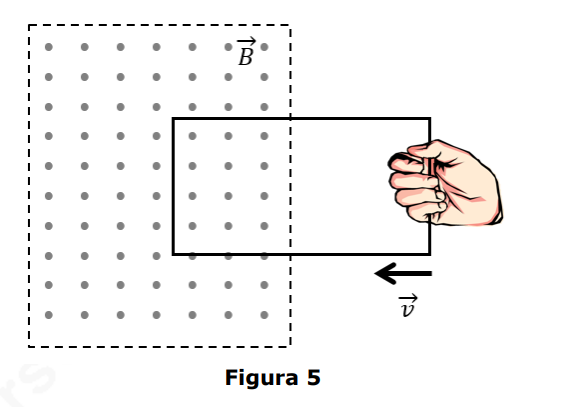
\includegraphics[scale=0.5]{figures/lei-faraday-lenz.png}
\end{figure}

Com base nesse contexto, a corrente elétrica induzida terá sentido \underline{\hspace{2cm}} na espira e a força magnética resultante atuará 
para \underline{\hspace{2cm}}.

Assinale a alternativa que preenche, correta e respectivamente, as lacunas do trecho acima.

\begin{itemize}
\item[(A)] horário - a esquerda
\item[(B)] anti-horário - a direita
\item[(C)] horário - a direita
\item[(D)] anti-horário - a esquerda
\item[(E)] anti-horário - fora do plano da página
\end{itemize}

\vspace{0.5cm}

\textcolor{red}{\textbf{Solução:}}\\

\textbf{1. Identificação do problema (variação do fluxo)}\\
O campo magnético $\vec{B}$ é orientado para \emph{fora} do plano (pontos). Ao inserir a espira para a esquerda, a área da espira 
que está dentro da região onde $\vec{B}$ existe aumenta. Portanto \colorbox{green!20}{o fluxo magnético $\Phi_B=\int \vec{B}\cdot d\vec{A}$ \emph{para fora}
do plano está aumentando com o tempo.}

\bigskip

\textbf{2. Aplicação da Lei de Lenz (sentido da corrente induzida)}\\
A Lei de Lenz afirma que a corrente induzida tem sentido tal que o campo magnético que ela gera se oponha à variação do fluxo que a produziu. Aqui o 
fluxo para fora do plano está \textbf{aumentando}; assim, a corrente induzida deve produzir um campo magnético \textbf{para dentro} \colorbox{green!30}{do plano 
(isto é, \emph{contrário} ao $\vec{B}$ externo) para tentar reduzir esse aumento.}

Para que o campo produzido por uma corrente circular seja dirigido \emph{para dentro} do plano (cruzes), o sentido da corrente, visto pelo observador, 
deve ser \textbf{horário}. (Regra da mão direita: dedos no sentido da corrente → polegar indica o sentido do campo no interior do laço.)

\bigskip

\textbf{3. Direção da força magnética resultante (oposição ao movimento)}\\
A corrente induzida estabelece forças magnéticas sobre os trechos da espira que estão imersos em $\vec{B}$. Considere o segmento vertical da espira que 
se encontra dentro da região do campo: com corrente no sentido horário, esse segmento vertical tem corrente para cima. \colorbox{green!30}{A força magnética(regra 
da m\~ao esquerda) sobre um fio} é dada por
\[
\vec{F}=I\,\vec{L}\times\vec{B}.
\]
Tomando $\vec{L}$ para cima e $\vec{B}$ para fora (para o observador), temos $\vec{L}\times\vec{B}$ apontando para a direita. 
Assim, a força magnética sobre esse segmento aponta para a direita, ou seja, \emph{oposta ao movimento de inserção da espira}, que 
é para a esquerda — exatamente o que exige a \colorbox{green!20}{Lei de Lenz (a força induzida tende a impedir a penetração).}

\bigskip

\textbf{4. Conclusão}\\
Portanto, a corrente induzida tem sentido \textbf{horário} e a força magnética resultante atua para a \textbf{direita}.

\textbf{Resposta:} \colorbox{green!50}{\textbf{C}}.

\end{flushleft}



\begin{flushleft}
\textbf{\textcolor{blue}{\Large Q}}\\
\noindent

\subsection{Quest\~ao }

\begin{itemize}
\item[(A)] 
\item[(B)] 
\item[(C)] 
\item[(D)] 
\item[(E)] 
\end{itemize}

\vspace{0.5cm}

\textcolor{red}{\textbf{Solução:}}\\

A resposta correta é alternativa \colorbox{green!50}{\textbf{...}}.
\end{flushleft}